\documentclass[10pt]{beamer}

\usetheme[progressbar=frametitle]{metropolis}
\usepackage{appendixnumberbeamer}

\usepackage{booktabs}
\usepackage[scale=2]{ccicons}

\usepackage{pgfplots}
\usepgfplotslibrary{dateplot}

\usepackage{xspace}
\newcommand{\themename}{\textbf{\textsc{metropolis}}\xspace}

\usepackage[english]{babel}
\usepackage{tikz}
\usepackage{pgfplots}
\usepackage{caption}
\usepackage{circuitikz}
\usepackage{listings}
\usepackage{pgfplotsthemetol}
\captionsetup{justification=centering}
\usetikzlibrary{plotmarks}
\usepackage[utf8]{inputenc}
\usepackage[english]{babel}
\usepackage{amsmath}
\usepackage{amsfonts}
\usepackage{amssymb}
\usepackage{graphicx}
\usepackage{setspace}
\usepackage{parskip}
\usepackage{amsthm}
\usepackage{fancyhdr}
\usepackage{booktabs}
\usepackage{hyperref}
\usepackage{pgfplots}% This uses tikz
\pgfplotsset{compat=newest}% use newest version
\usepackage{sidecap}
\usepackage{tikz}
\usepackage{tikz-3dplot}
\usepackage{xcolor}
\usepackage{xstring}
\usepackage{multirow}
\usepackage{adjustbox}

\usepackage{caption}
\usepackage{color}
\usepackage{array}
\usepackage{wrapfig}
\usepackage{listings}

\captionsetup{justification=centering}
\usetikzlibrary{plotmarks}

\usepackage{lipsum}% http://ctan.org/pkg/lipsum
\usepackage{hanging}% http://ctan.org/pkg/hanging


\usepackage[scale=2]{ccicons}
\usepackage{minted}

\usemintedstyle{trac}
\definecolor{mDarkTeal}{HTML}{23373b}
\setbeamercolor{section page}{bg=mDarkTeal}

%*******************************************************************************

\title{VRIC: Variable Rate Image Compression with Recurrent Neural Networks}
\subtitle{Coding of Audiovisual Contents}
\date{Barcelona, \today}
\author{Miquel Oller Oliveras \& Alvaro Scherk Fontanals}
\institute{ \vspace{40pt} 
\includegraphics[height=20pt]{./img/logoUPC.png}\hspace{75pt}
\includegraphics[height=20pt]{./img/etsetb3.png}}

%*******************************************************************************
\begin{document}

\maketitle

\begin{frame}{Table of Contents:}
  \tableofcontents
\end{frame}


% SECTION 1: ======================================================================

\begingroup
\setbeamercolor{section title}{fg=white}
\setbeamercolor{background canvas}{bg=mDarkTeal}
\section{VRIC: An overview of the proposal}
\endgroup


% SLIDE 1: _____________________________________________________________________
\begin{frame}{An overview of the proposal: Abstract\footnotemark}
\centering
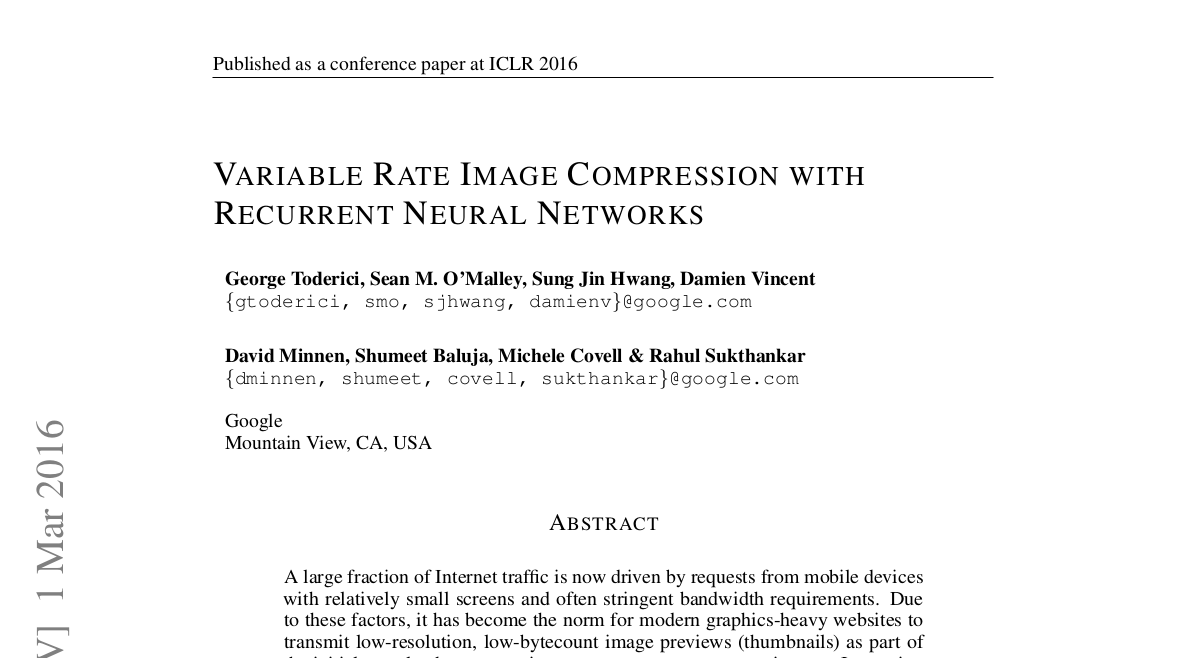
\includegraphics[width =0.5\linewidth]{./img/VRIC_paper.png}
  \begin{itemize}
    \item Low-resolution thumbnail images
    \item Variable fixed encoding size
    \item Standards do not perform well with low-dimentional images
    \item Fresh air into image encoding world
    \item Trained end-to-end
  \end{itemize}
  \begin{figure}
    \begin{minipage}{\textwidth}
            \footnotetext{[1] Proposal by George Toderici et al. All from the Google, Mountain View, CA, USA. Published in ICLR 2016} \\
    \end{minipage}
\end{figure}
\end{frame}




% SECTION 2:====================================================================

\begingroup
\setbeamercolor{section title}{fg=white}
\setbeamercolor{background canvas}{bg=mDarkTeal}
\section{Neural Networks Overview}
\endgroup

% SLIDE : _____________________________________________________________________
\begin{frame}{Neural Networks Overview: General Knowledge}
  Basic perceptron Scheme:
  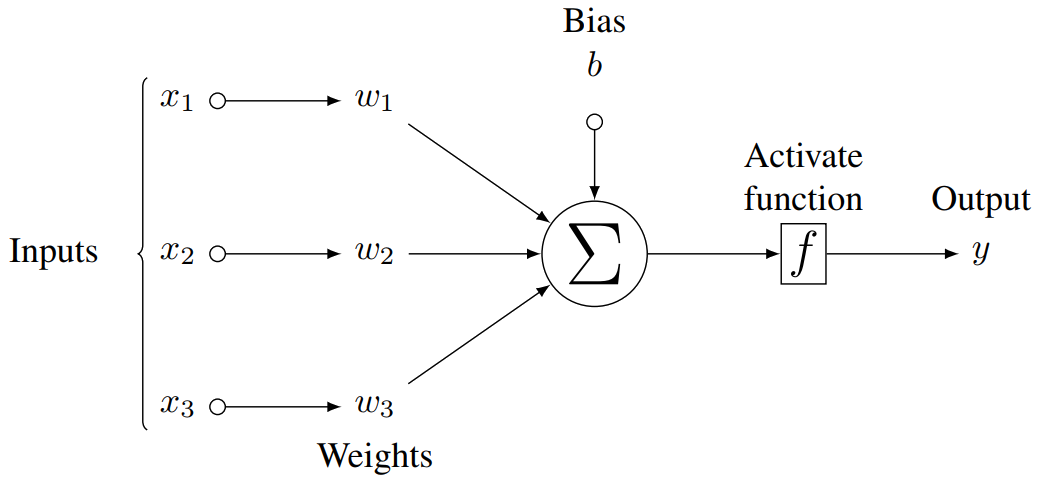
\includegraphics[width=0.9\linewidth]{./img/perceptron.png}


\begin{equation*}
  \begin{bmatrix}y_1\\ y_2 \\ \vdots \\ y_{m} \end{bmatrix} =
 \begin{bmatrix}
 w_{11} & w_{12} & \cdots & w_{1n}\\
 w_{21} & w_{22} & \cdots & w_{2n}\\
 \vdots & \vdots & \ddots & \vdots \\
  w_{m1} & w_{m2} & \cdots & w_{mn}\\
 \end{bmatrix}
 \begin{bmatrix}x_1 \\ x_2 \\ \vdots \\ x_n \end{bmatrix}
 + \begin{bmatrix}b_1 \\ b_2 \\ \vdots \\ b_m \end{bmatrix}
\end{equation*}

\end{frame}






% SLIDE : _____________________________________________________________________
\begin{frame}{Neural Networks Overview: Auto-Encoder}
  \vspace{5mm}
  Auto-Encoder Basic Scheme:\\
  \vspace{5mm}
  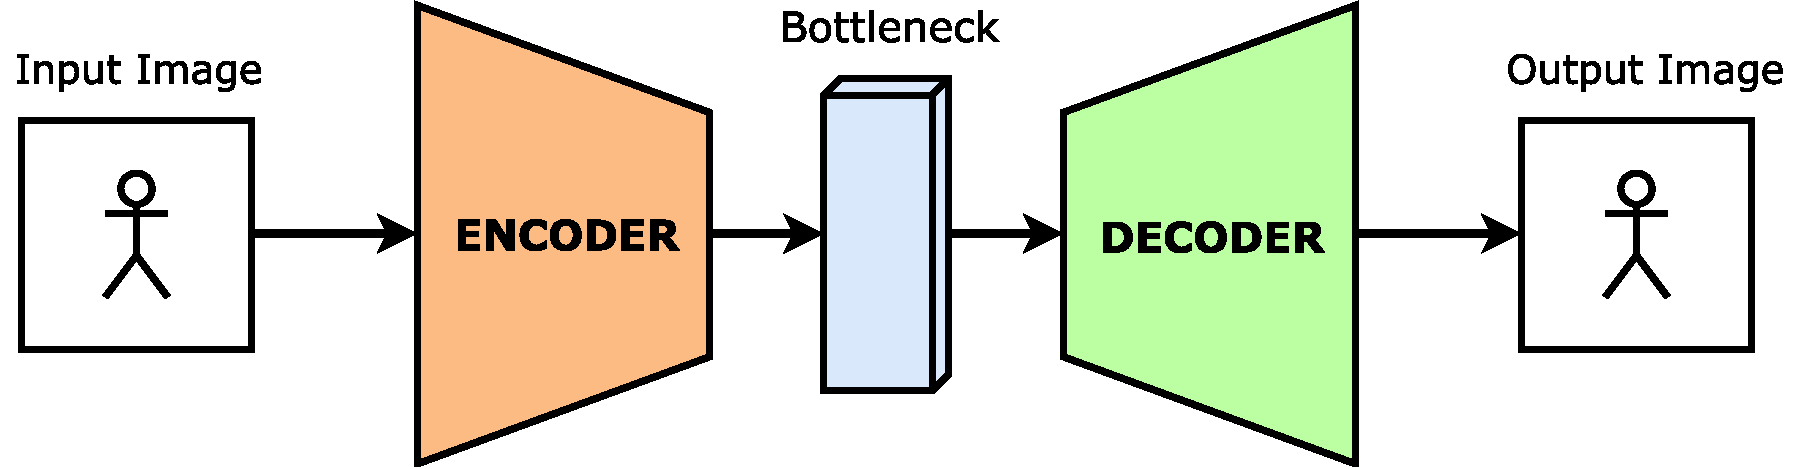
\includegraphics[width=\linewidth]{./img/autoencoder1.pdf}
  \vspace{20mm}
  \begin{figure}
    \begin{minipage}{\textwidth}
            \footnotetext{[2] Depicted as images but any type of data can be used as input} \\
    \end{minipage}
\end{figure}
\end{frame}




% SECTION 3:====================================================================

\begingroup
\setbeamercolor{section title}{fg=white}
\setbeamercolor{background canvas}{bg=mDarkTeal}
\section{Architectures and Schematics}
\endgroup

% SLIDE : _____________________________________________________________________
\begin{frame}{Architectures and Schematics: General Scheme}
  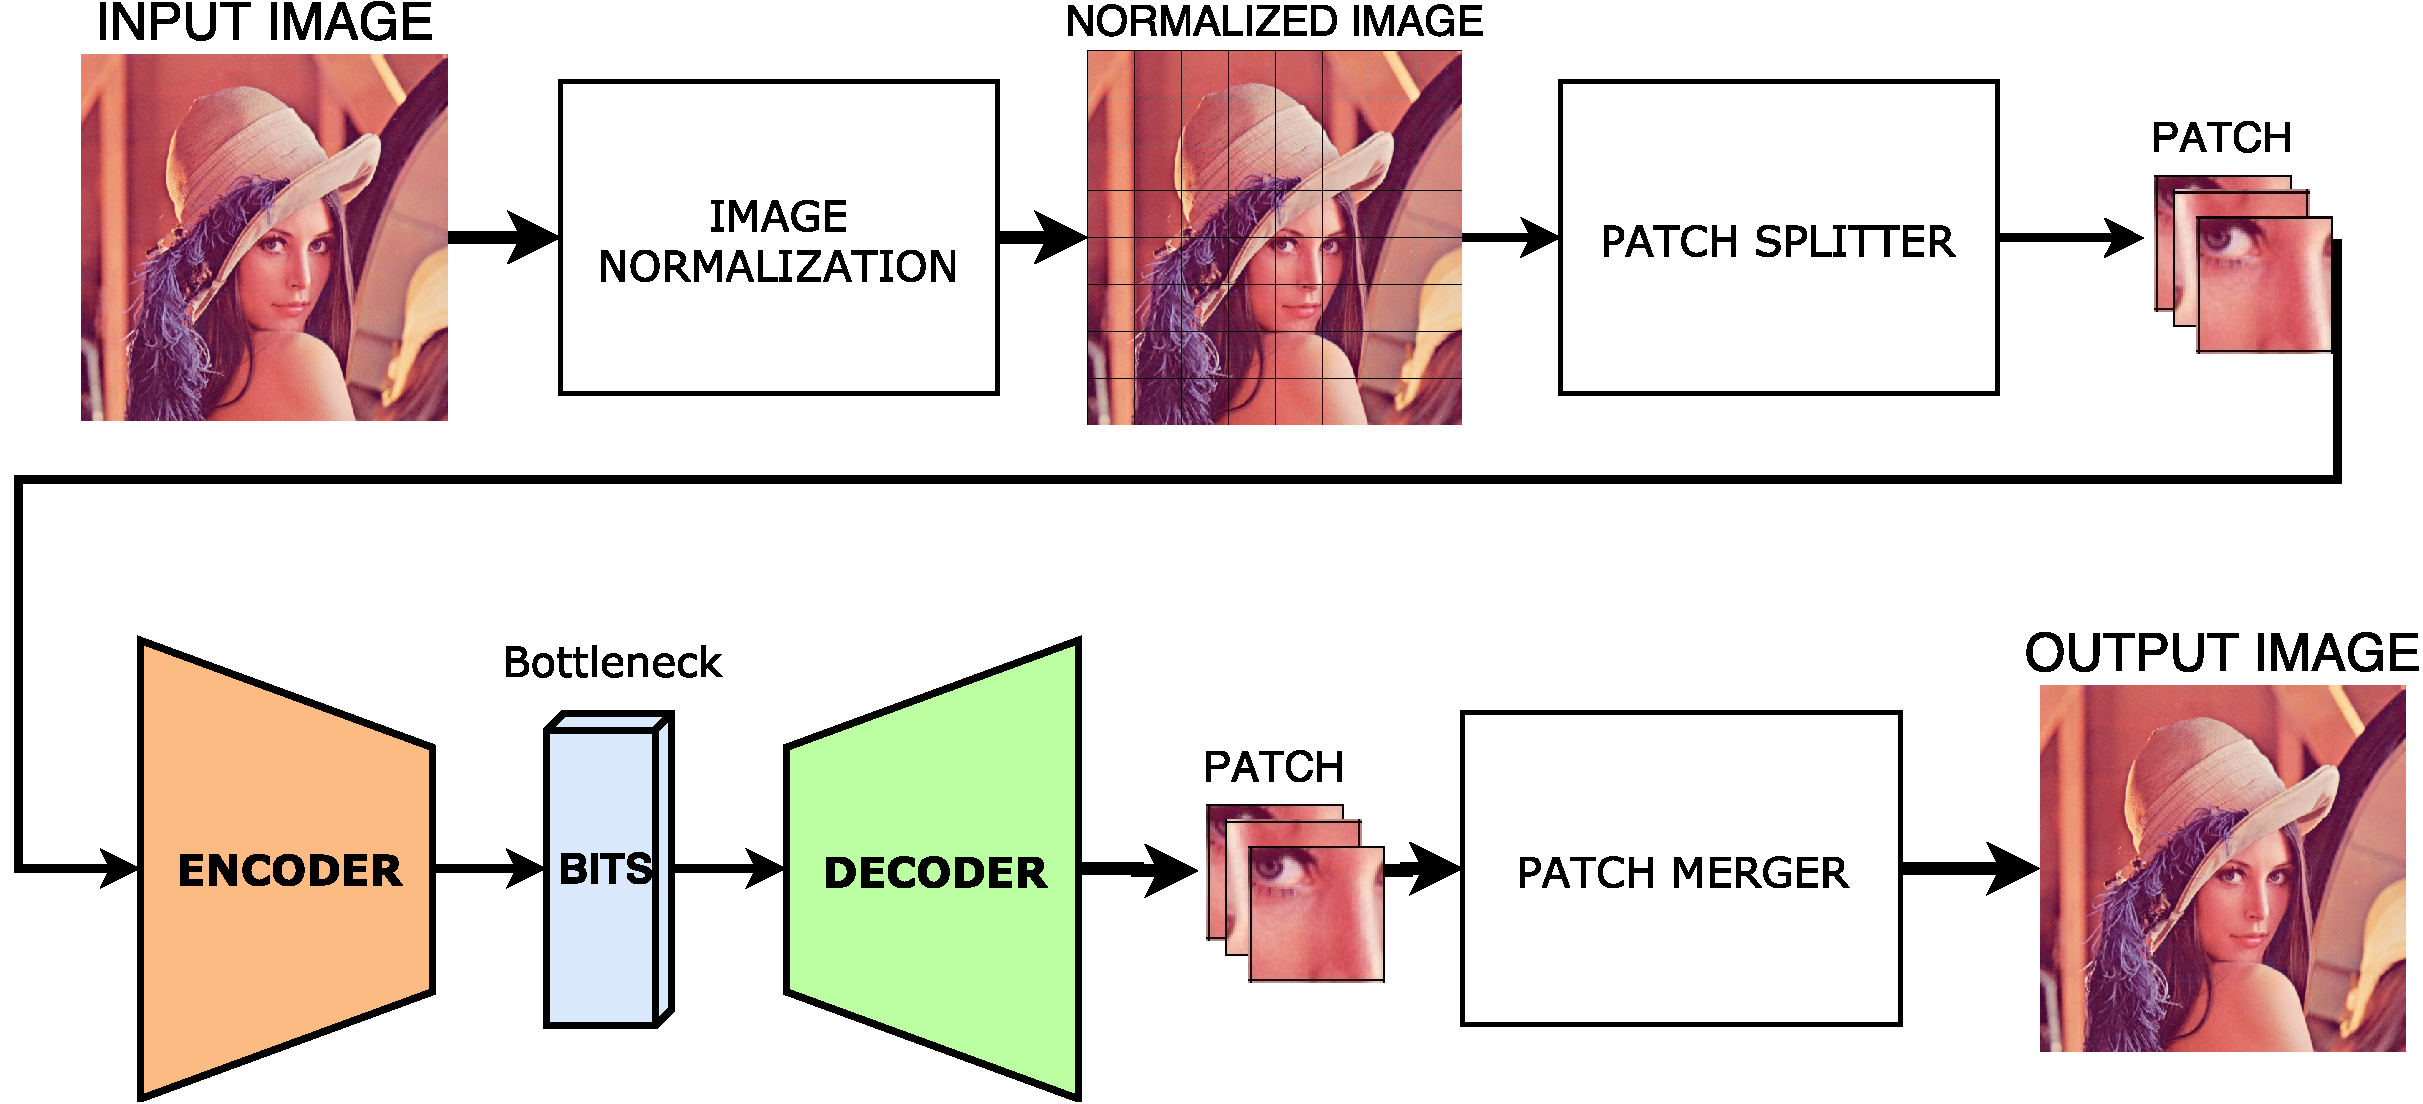
\includegraphics[width=\linewidth]{./img/generalScheme.pdf}
\end{frame}


% SLIDE : ____________________________________________________________________
\begin{frame}{Architectures and Schematics: Straight-Forward FC }
      Encoder:
      \begin{center}
        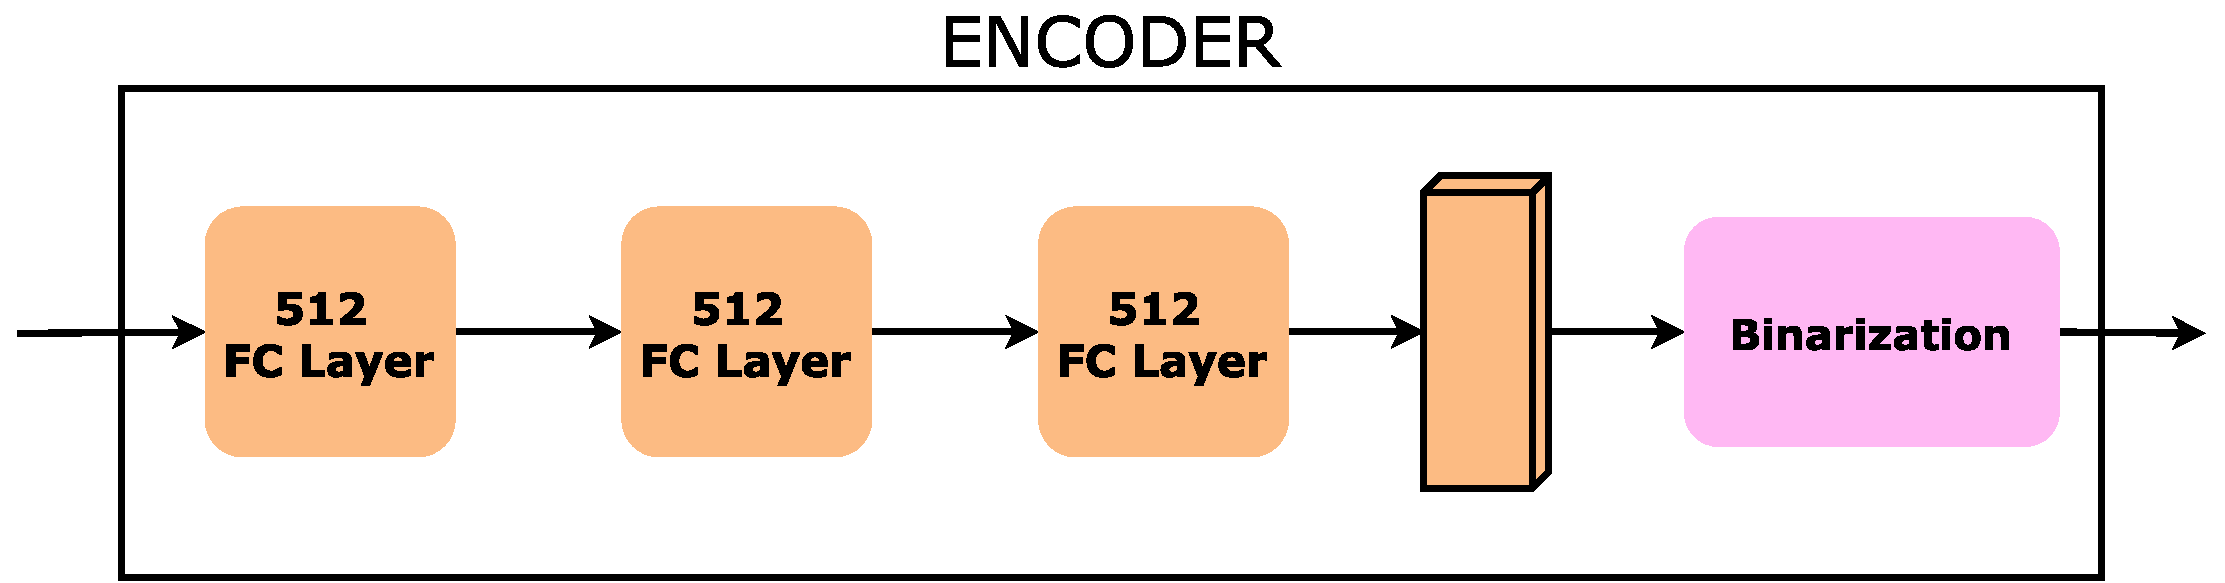
\includegraphics[height=20mm]{./img/FCencoder.pdf}
      \end{center}
      Decoder:
      \begin{center}
        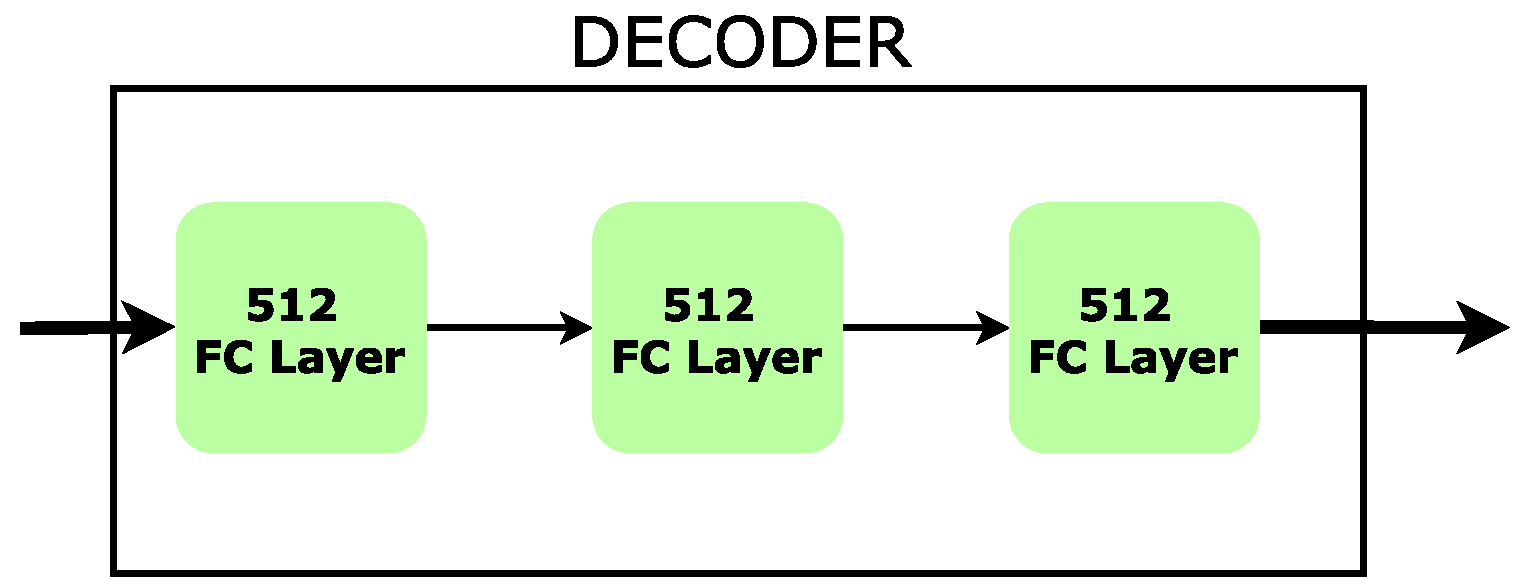
\includegraphics[height=20mm]{./img/FCdecoder.pdf}
      \end{center}
      Straight-Forward Scheme:
      \begin{center}
      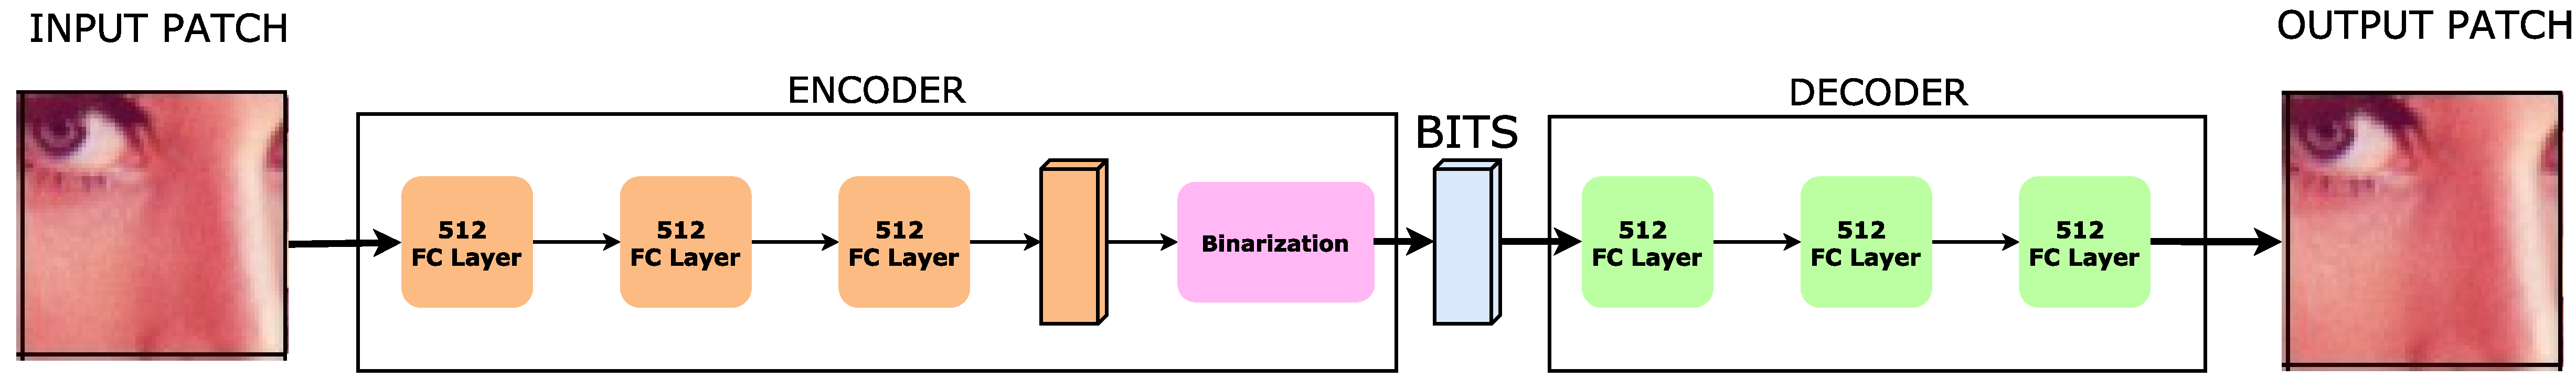
\includegraphics[width=\linewidth]{./img/Straighfroward_FC_Scheme.pdf}
      \end{center}
\end{frame}
% SLIDE : _____________________________________________________________________
\begin{frame}{Architectures and Schematics: Binary Layer}
  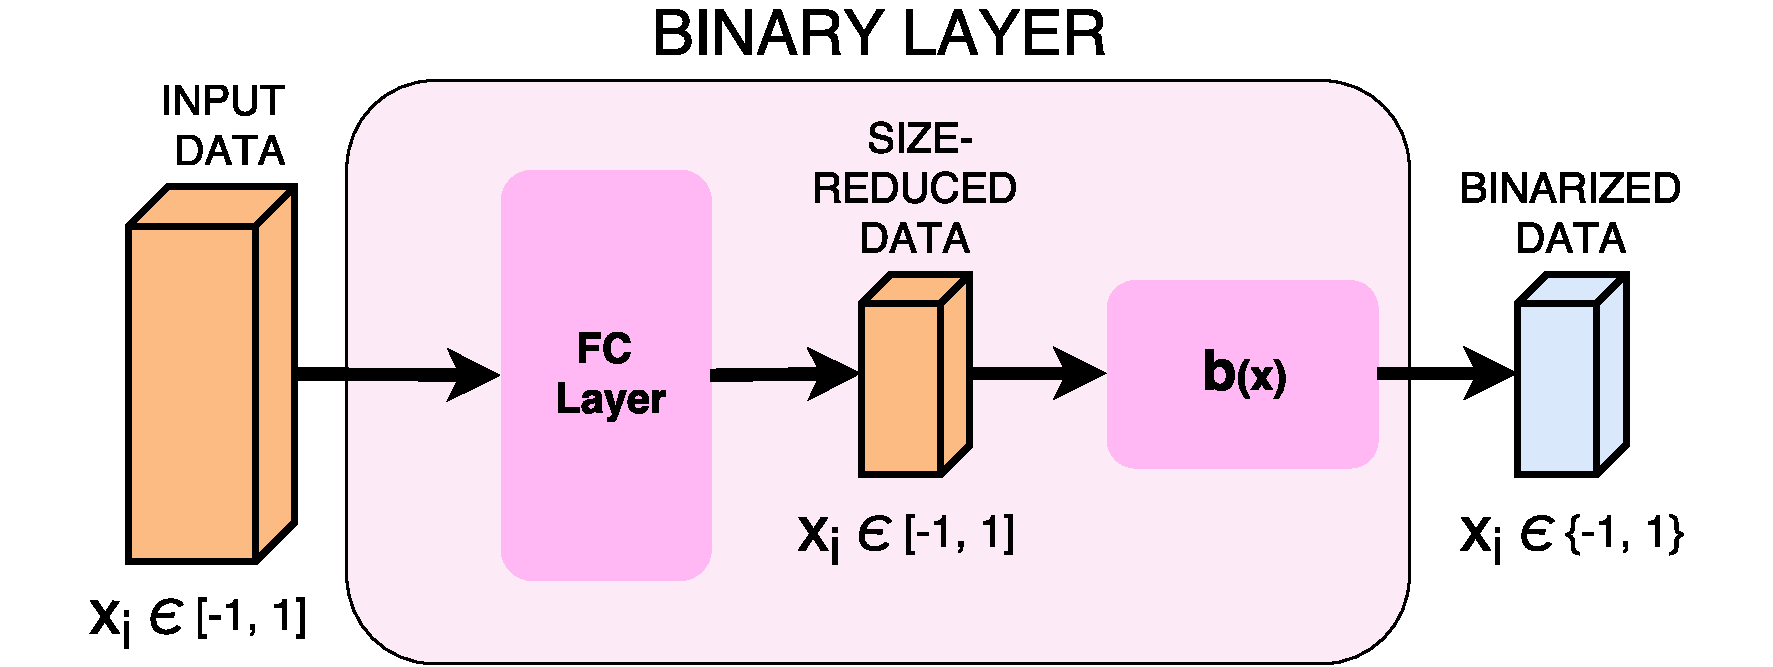
\includegraphics[width=\linewidth]{./img/binarizator.pdf}
  \begin{equation*}
    b(x) = x + \epsilon \ \in \{-1,1\}
  \end{equation*}
  \begin{equation*}
    \epsilon \sim \begin{cases} +1 - x & \mbox{with probability } \frac{1+x}{2}, \\ -x - 1 & \mbox{with probability } \frac{1-x}{2}.\end{cases}
  \end{equation*}
  \begin{figure}
    \begin{minipage}{\textwidth}
            \footnotetext{[3] Method proposed by: Raiko, Tapani, et al. “Techniques for Learning Binary Stochastic Feedforward Neural Networks.” [1406.2989] ICLR 2015, 9 Apr. 2015, arxiv.org/abs/1406.2989} \\
    \end{minipage}
  \end{figure}

\end{frame}

% SLIDE : ____________________________________________________________________
\begin{frame}{Architectures and Schematics:  Residual FC }
    Encoding Scheme:\\
    \vspace{5mm}
      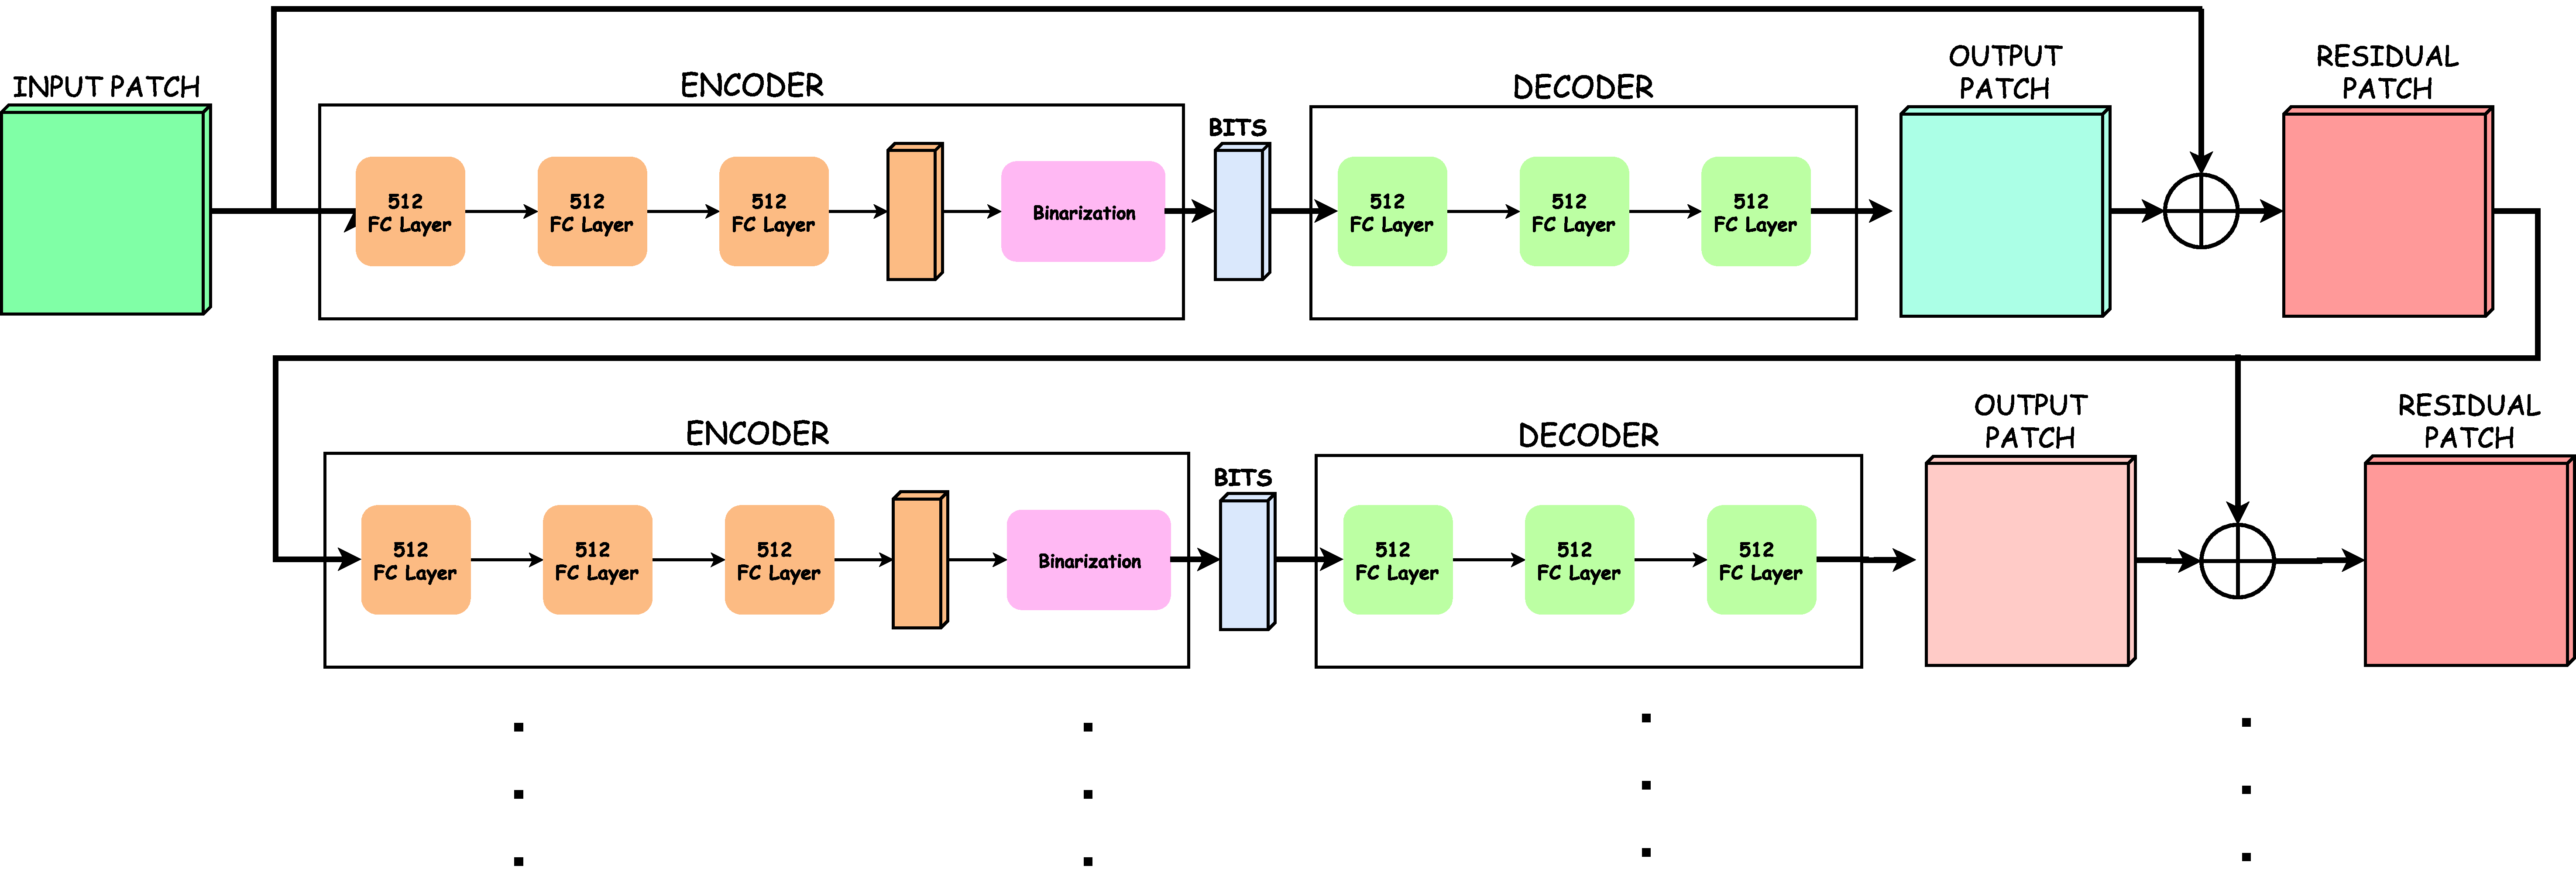
\includegraphics[width=1.05\linewidth]{./img/encodingScheme.pdf}

      \vspace{20mm}
      \begin{figure}
        \begin{minipage}{\textwidth}
                \footnotetext{[4] Using $\tanh$ non-linearities in all layers} \\
        \end{minipage}
    \end{figure}
\end{frame}
% SLIDE : ____________________________________________________________________
\begin{frame}{Architectures and Schematics: Residual FC }
  Decoding Scheme:\\
      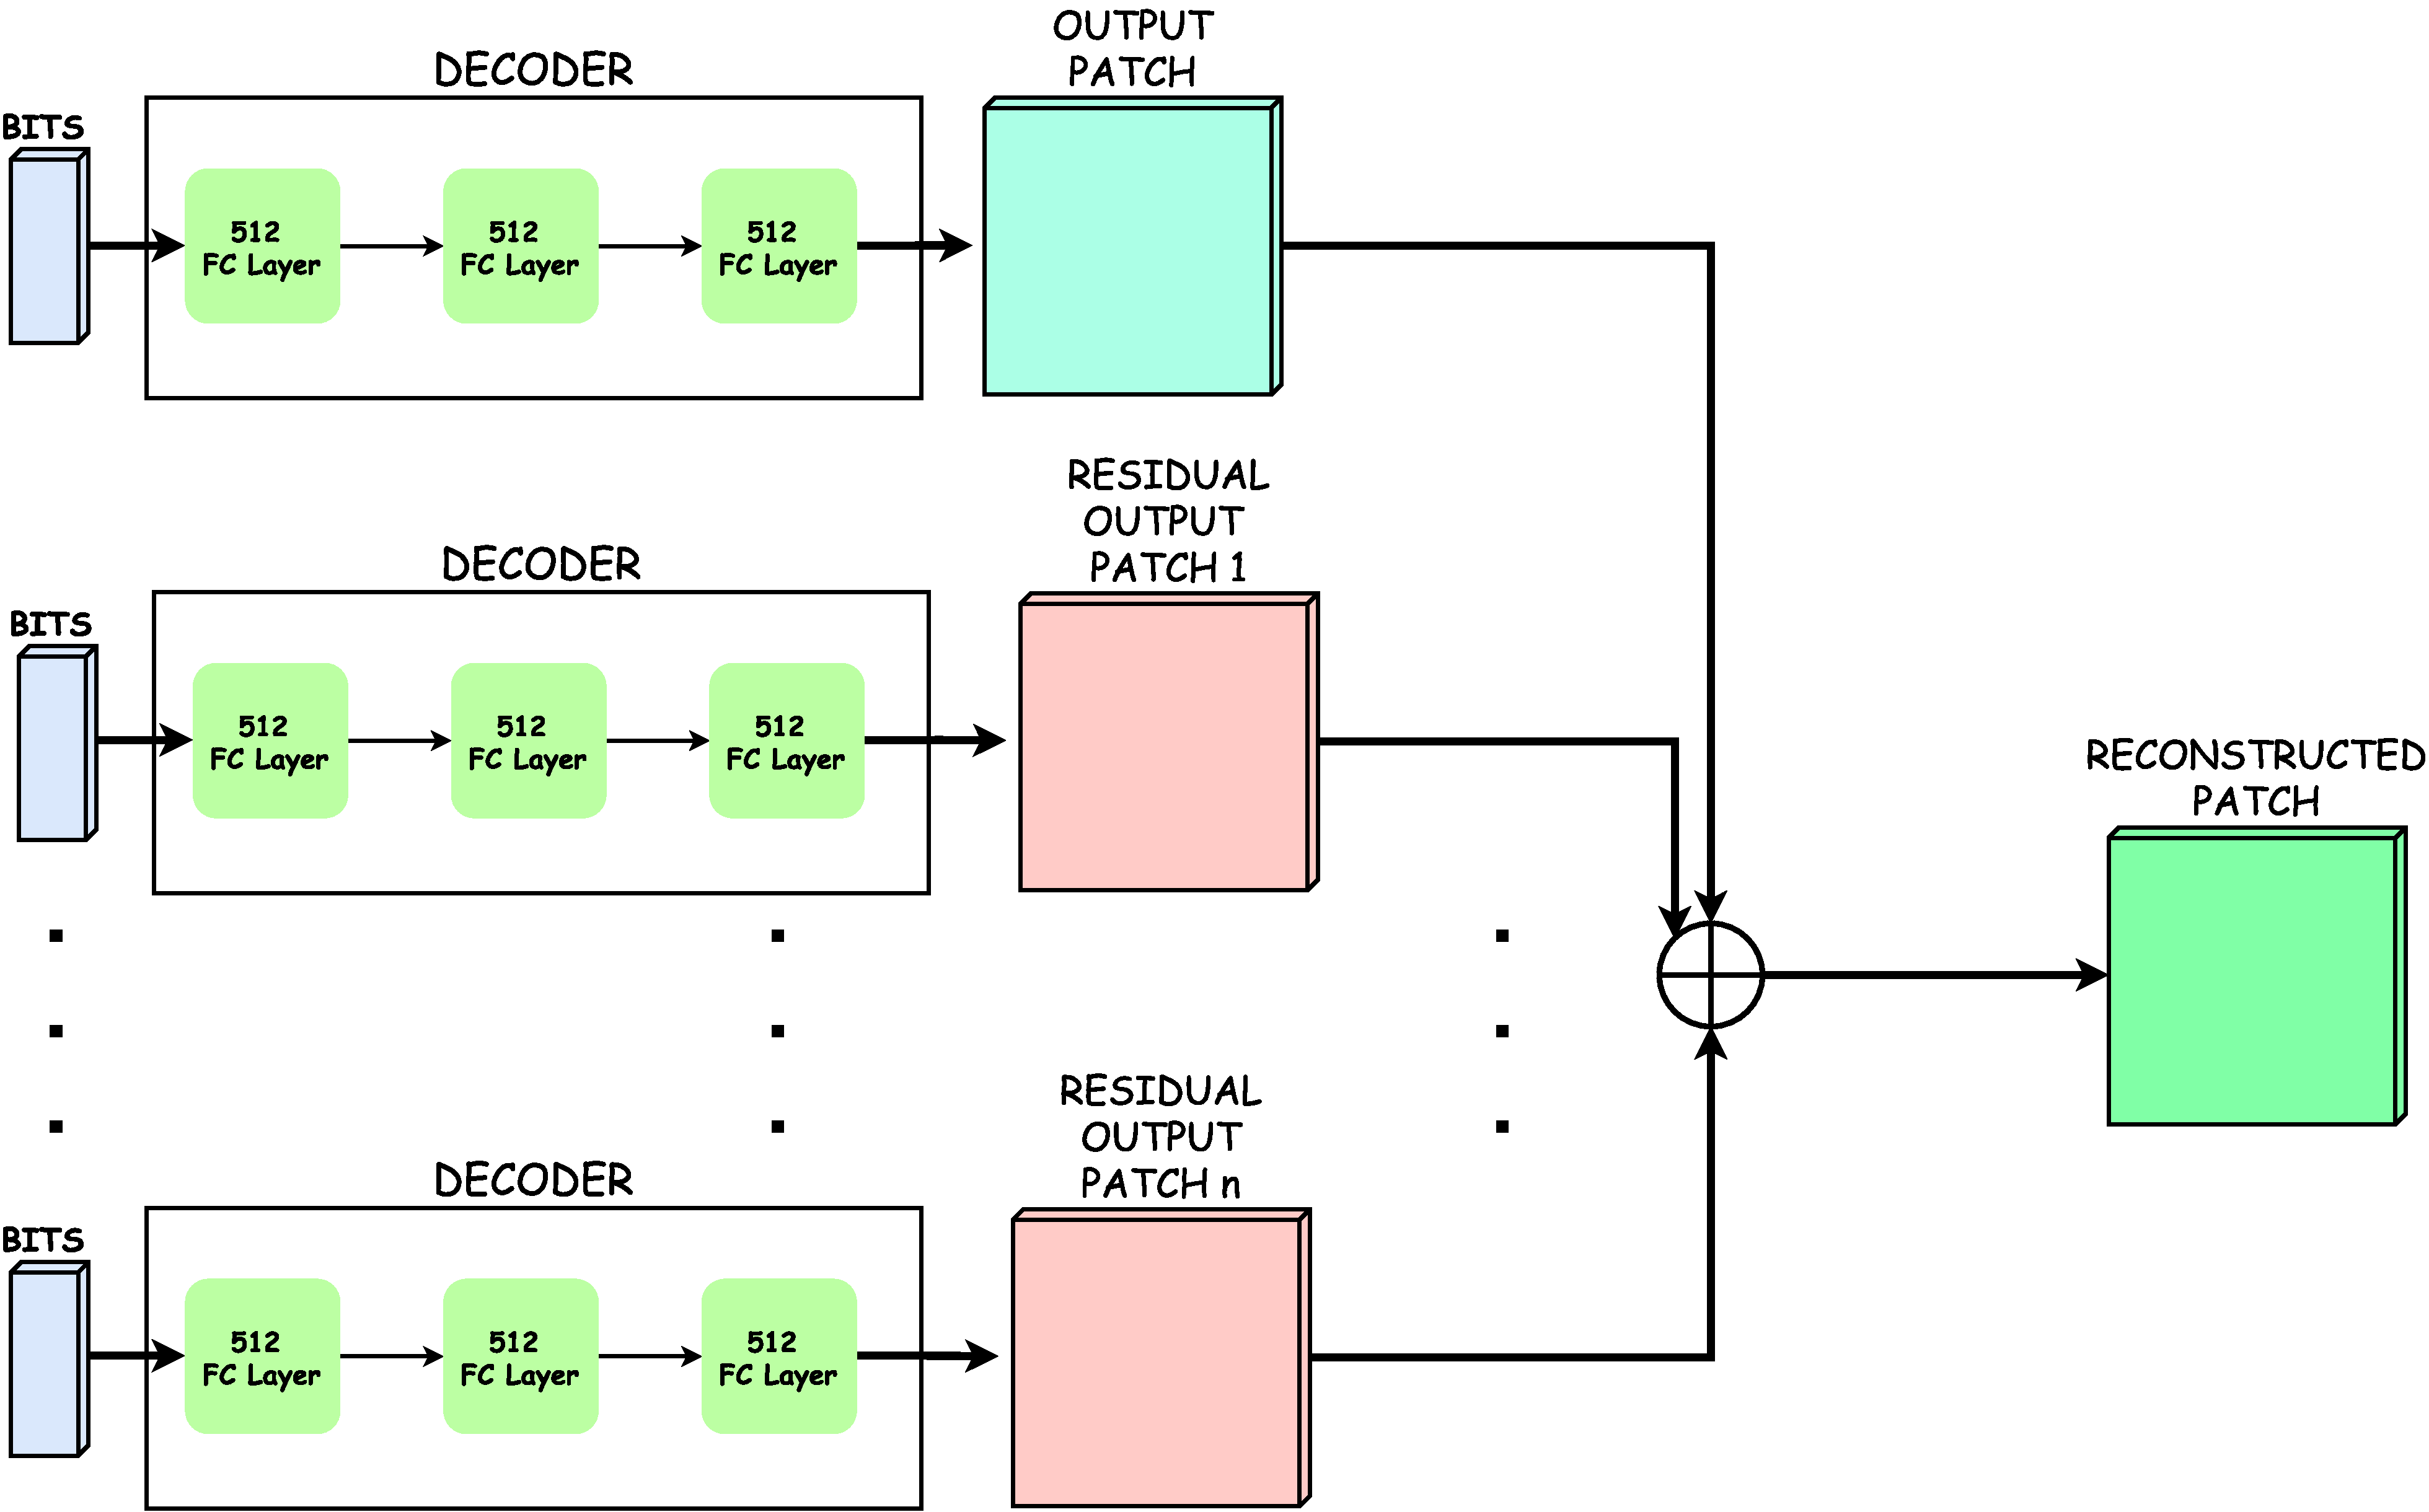
\includegraphics[width=\linewidth]{./img/reconstruction.pdf}
\end{frame}


% SLIDE : _____________________________________________________________________
\begin{frame}{Architectures and Schematics: LSTM Based Scheme}
  Encoder Block:
  \begin{center}
    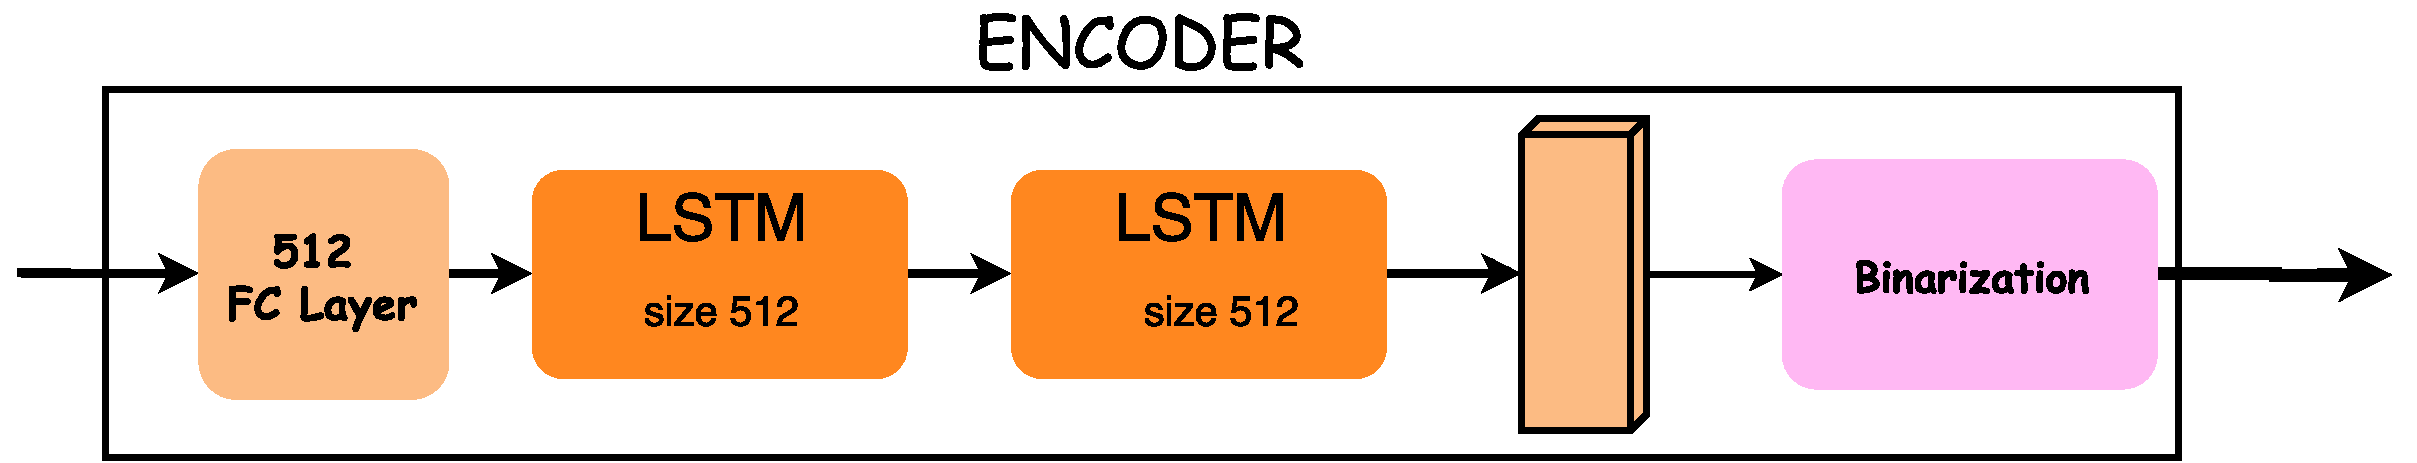
\includegraphics[height=20mm]{./img/LSTM_encoder_block.pdf}
  \end{center}
  Decoder Block:
  \begin{center}
    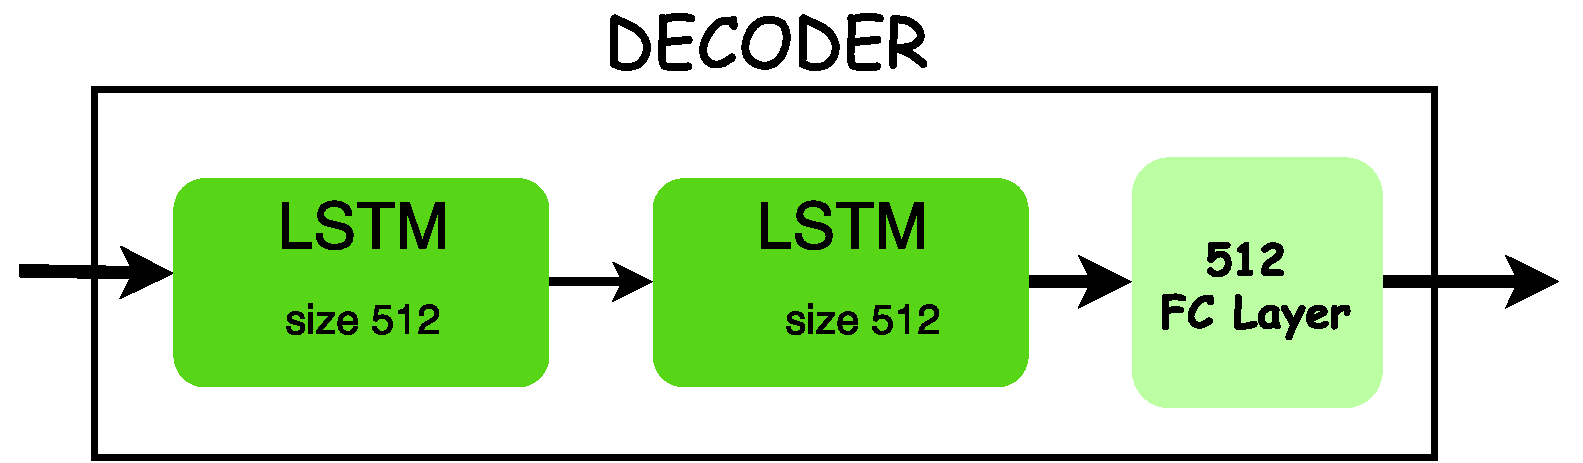
\includegraphics[height=20mm]{./img/LSTM_decoder_block.pdf}
  \end{center}
\end{frame}
% SLIDE : _____________________________________________________________________
\begin{frame}{Architectures and Schematics: LSTM Based Scheme}
  Encoder:\\
  \vspace{1mm}
  \begin{center}
    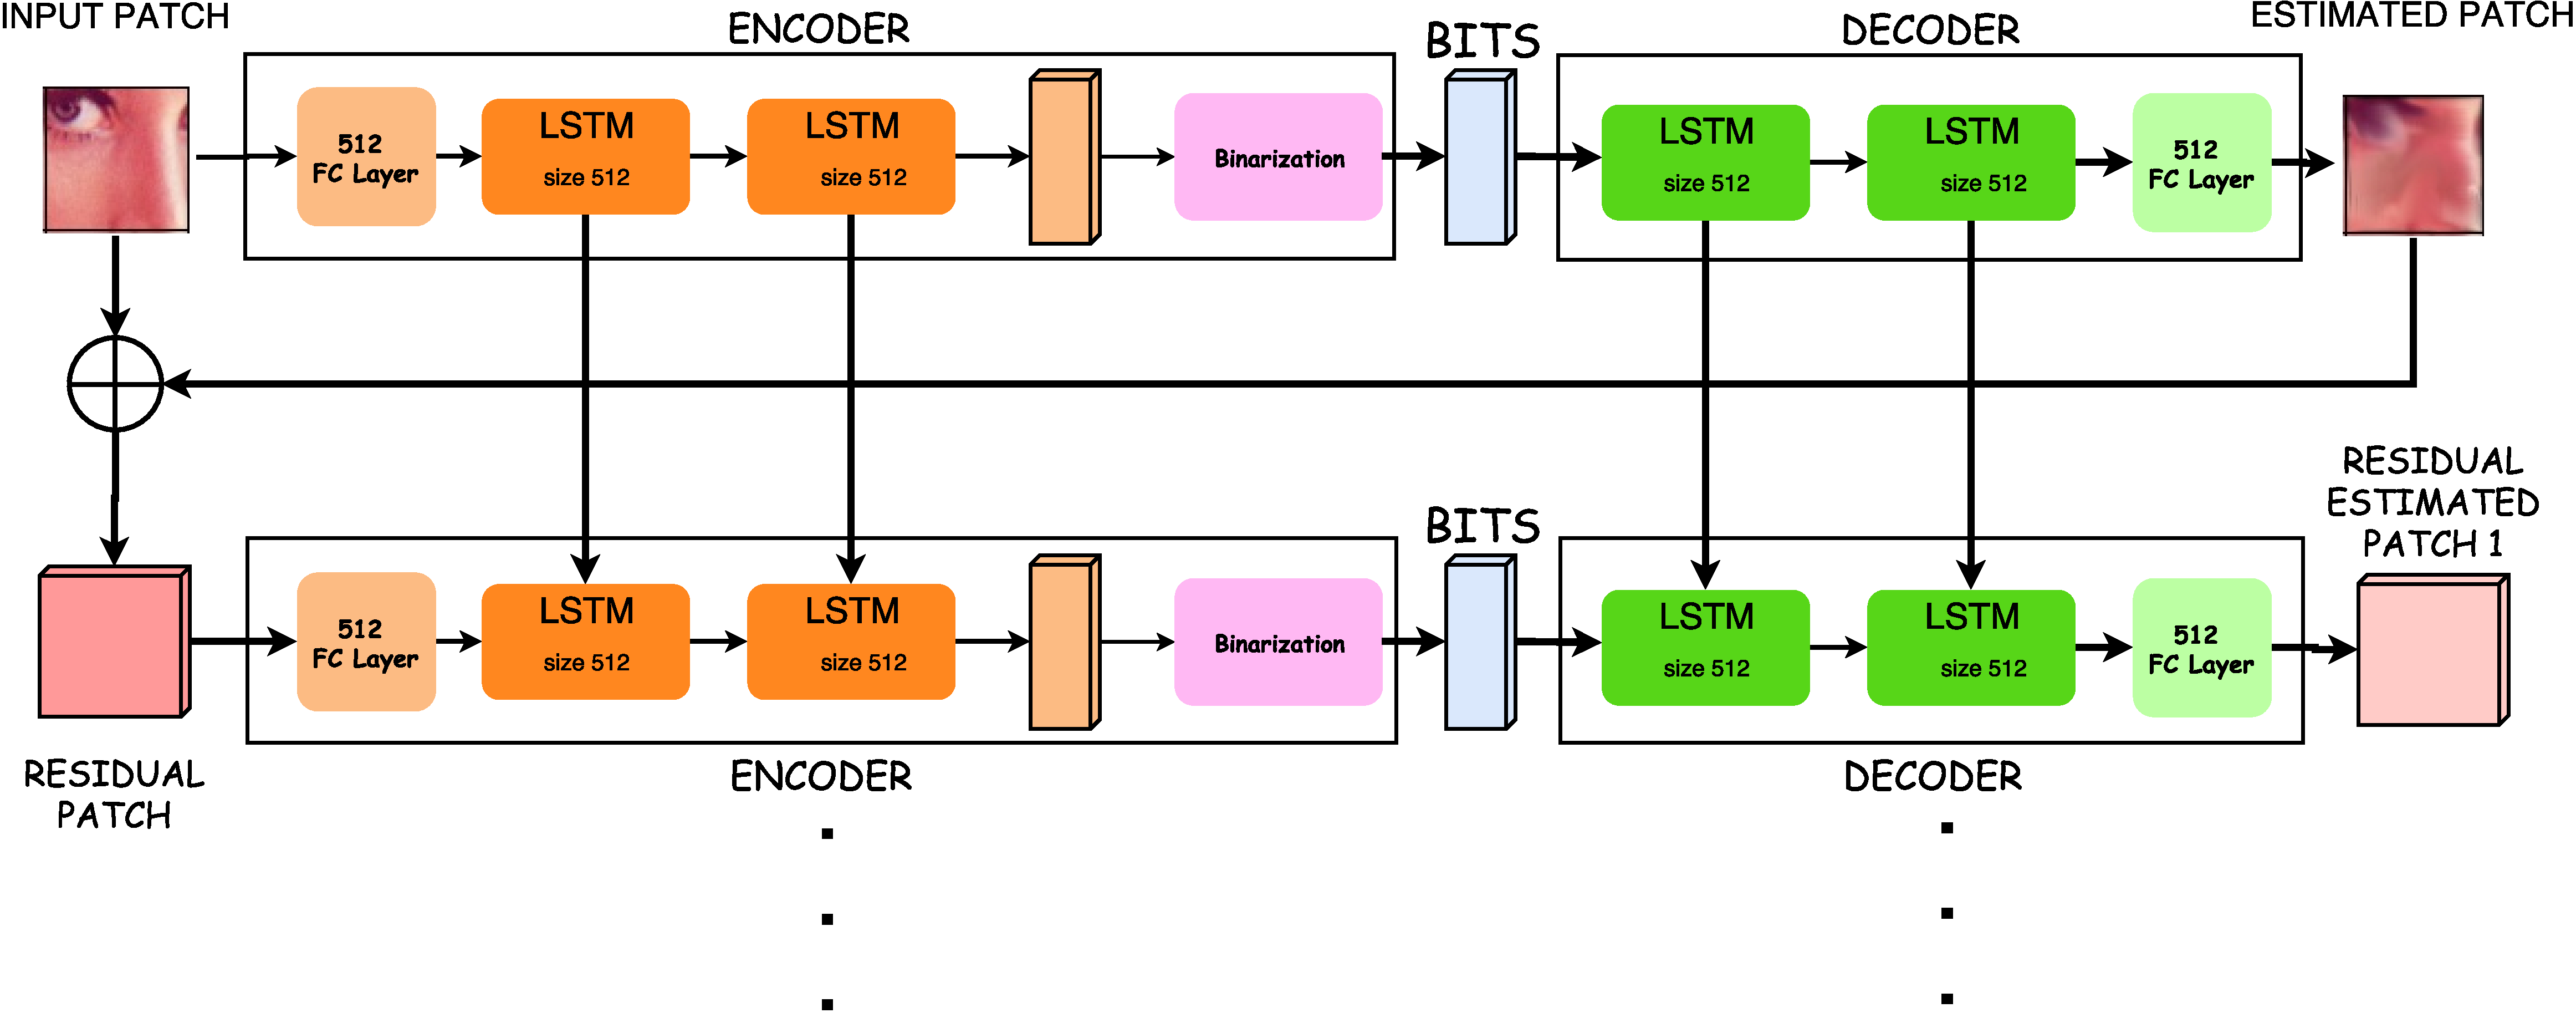
\includegraphics[width=\linewidth]{./img/LSTM_Scheme.pdf}
  \end{center}
  \vspace{15mm}
  \begin{figure}
    \begin{minipage}{\textwidth}
            \footnotetext{[5] Using $\tanh$ non-linearities in all layers} \\
    \end{minipage}
\end{figure}
\end{frame}
% SLIDE : _____________________________________________________________________
\begin{frame}{Architectures and Schematics: LSTM Based Scheme}
  Decoder:
  \begin{center}
    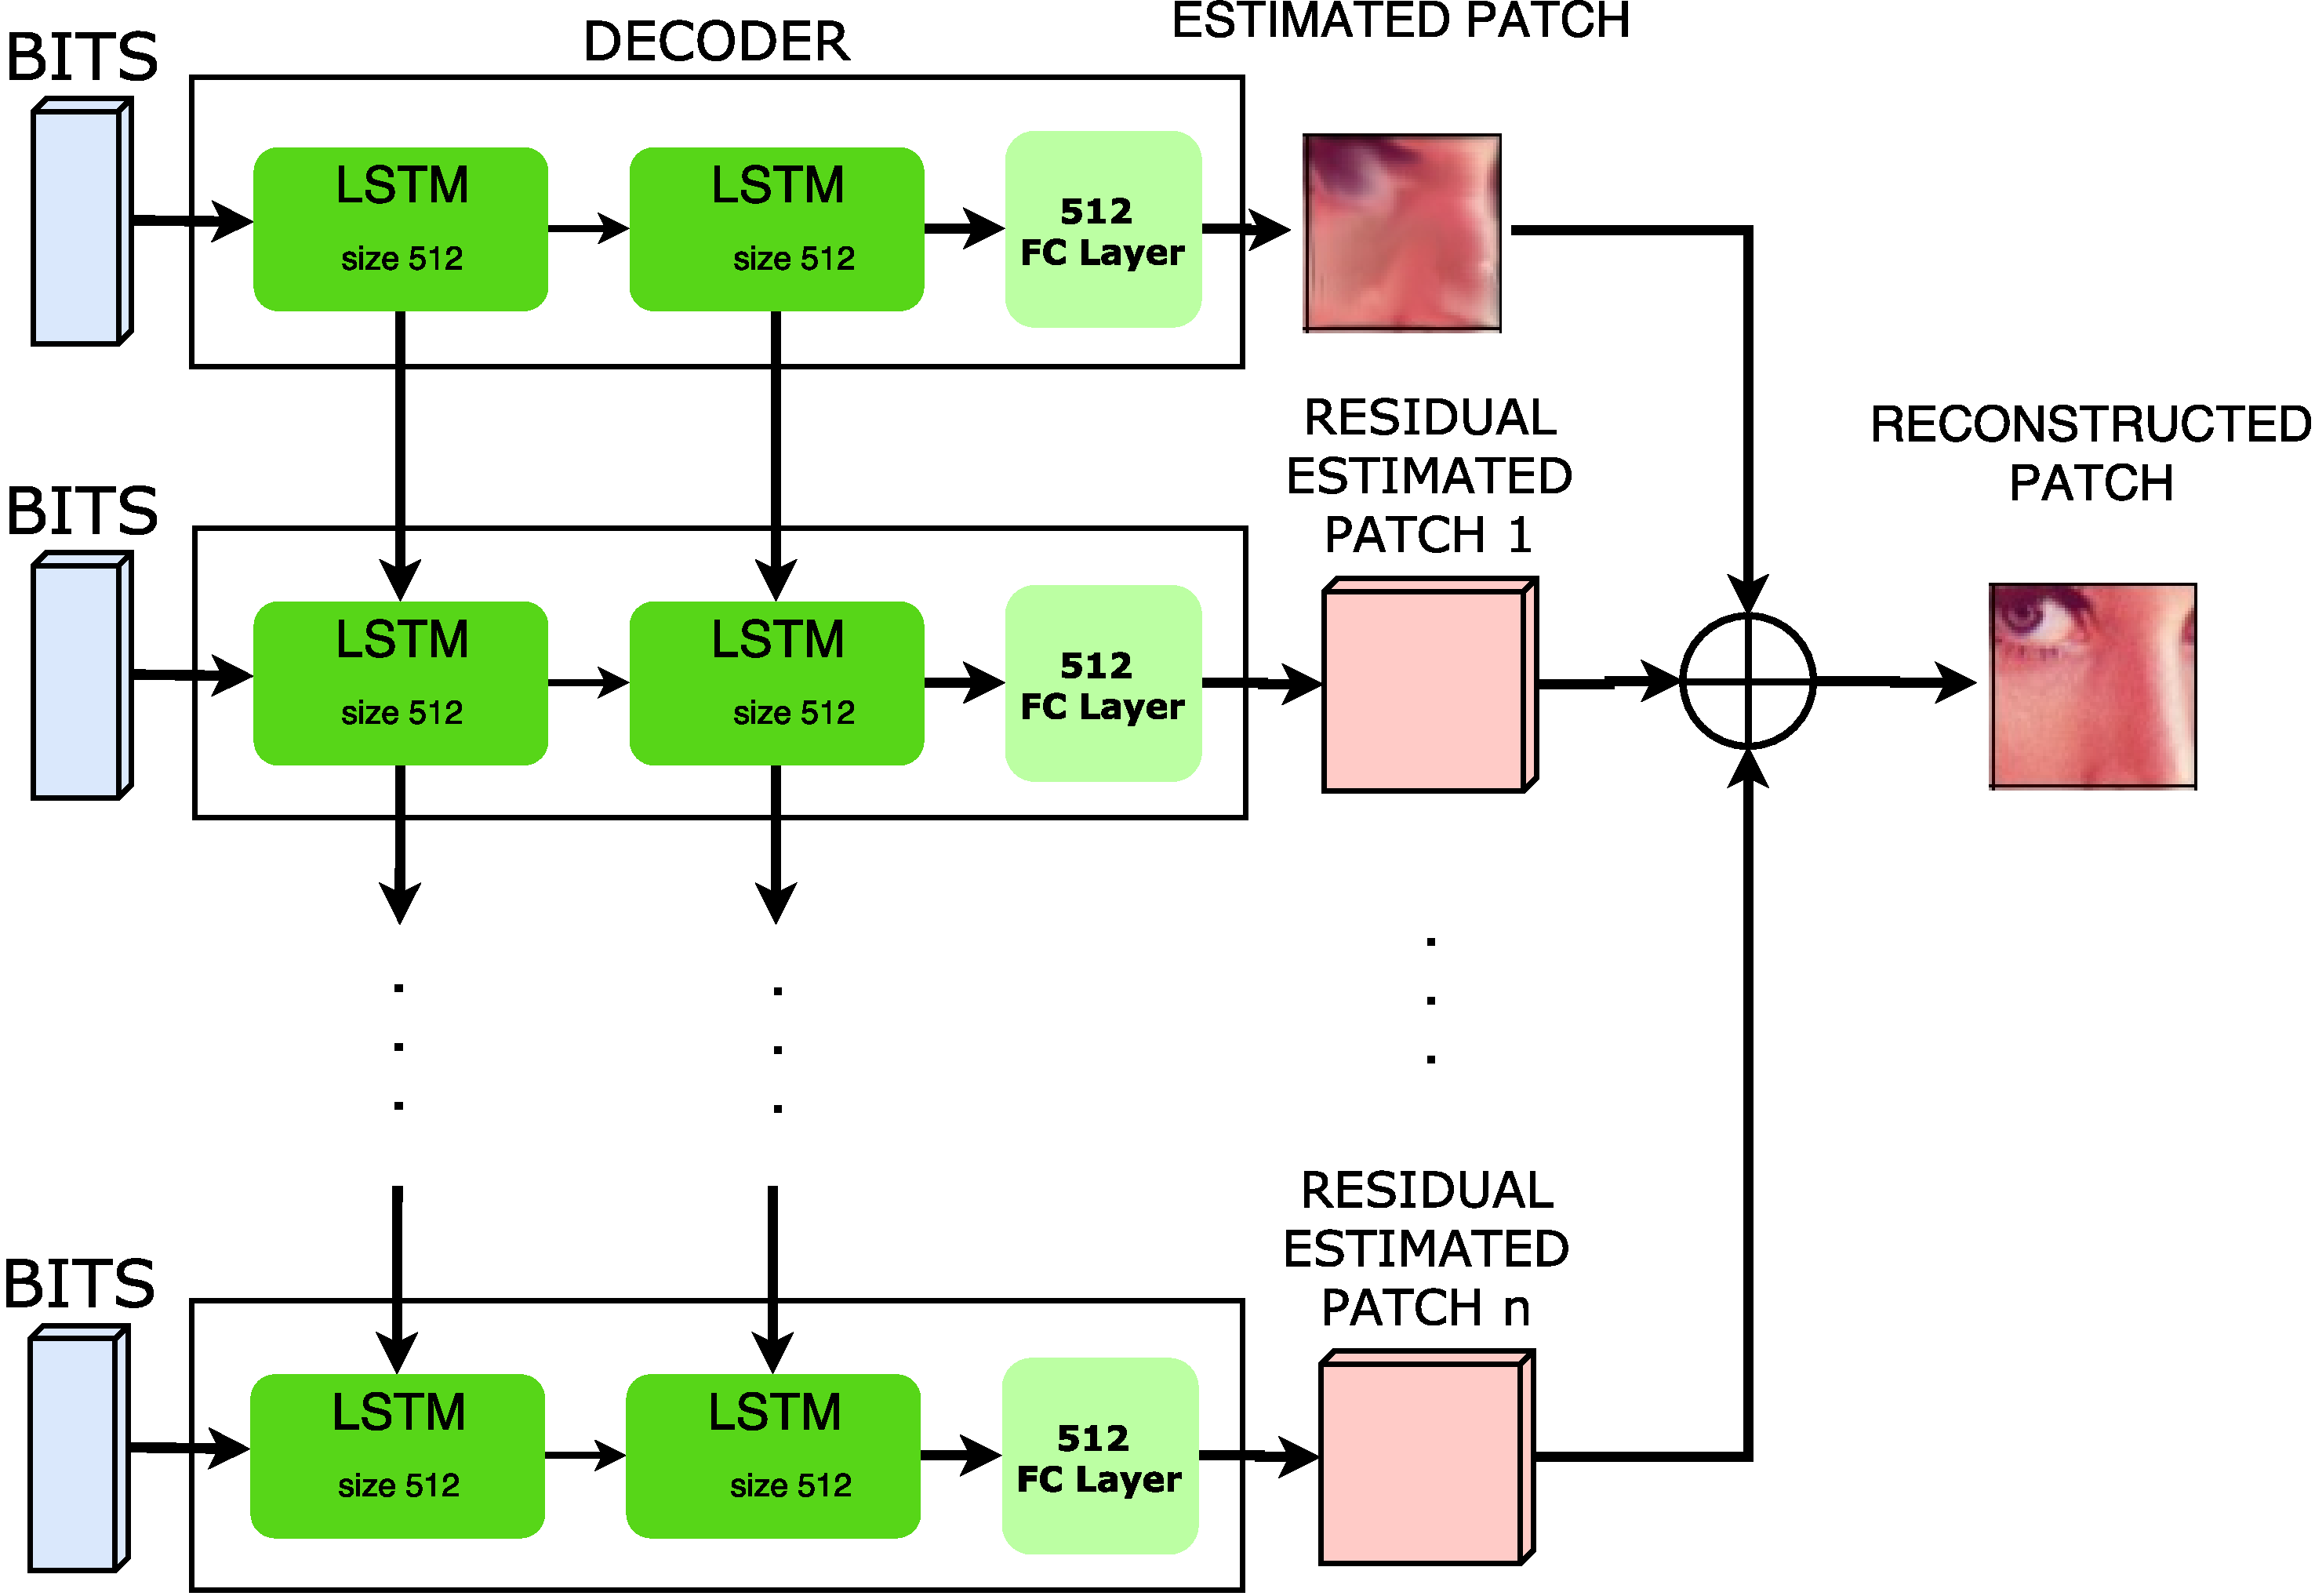
\includegraphics[width=\linewidth]{./img/LSTM_global_decoder.pdf}
  \end{center}
\end{frame}

% SLIDE : _____________________________________________________________________
\begin{frame}{Architectures and Schematics: Our LSTM Proposed Scheme}
  Decoder:
  \begin{center}
    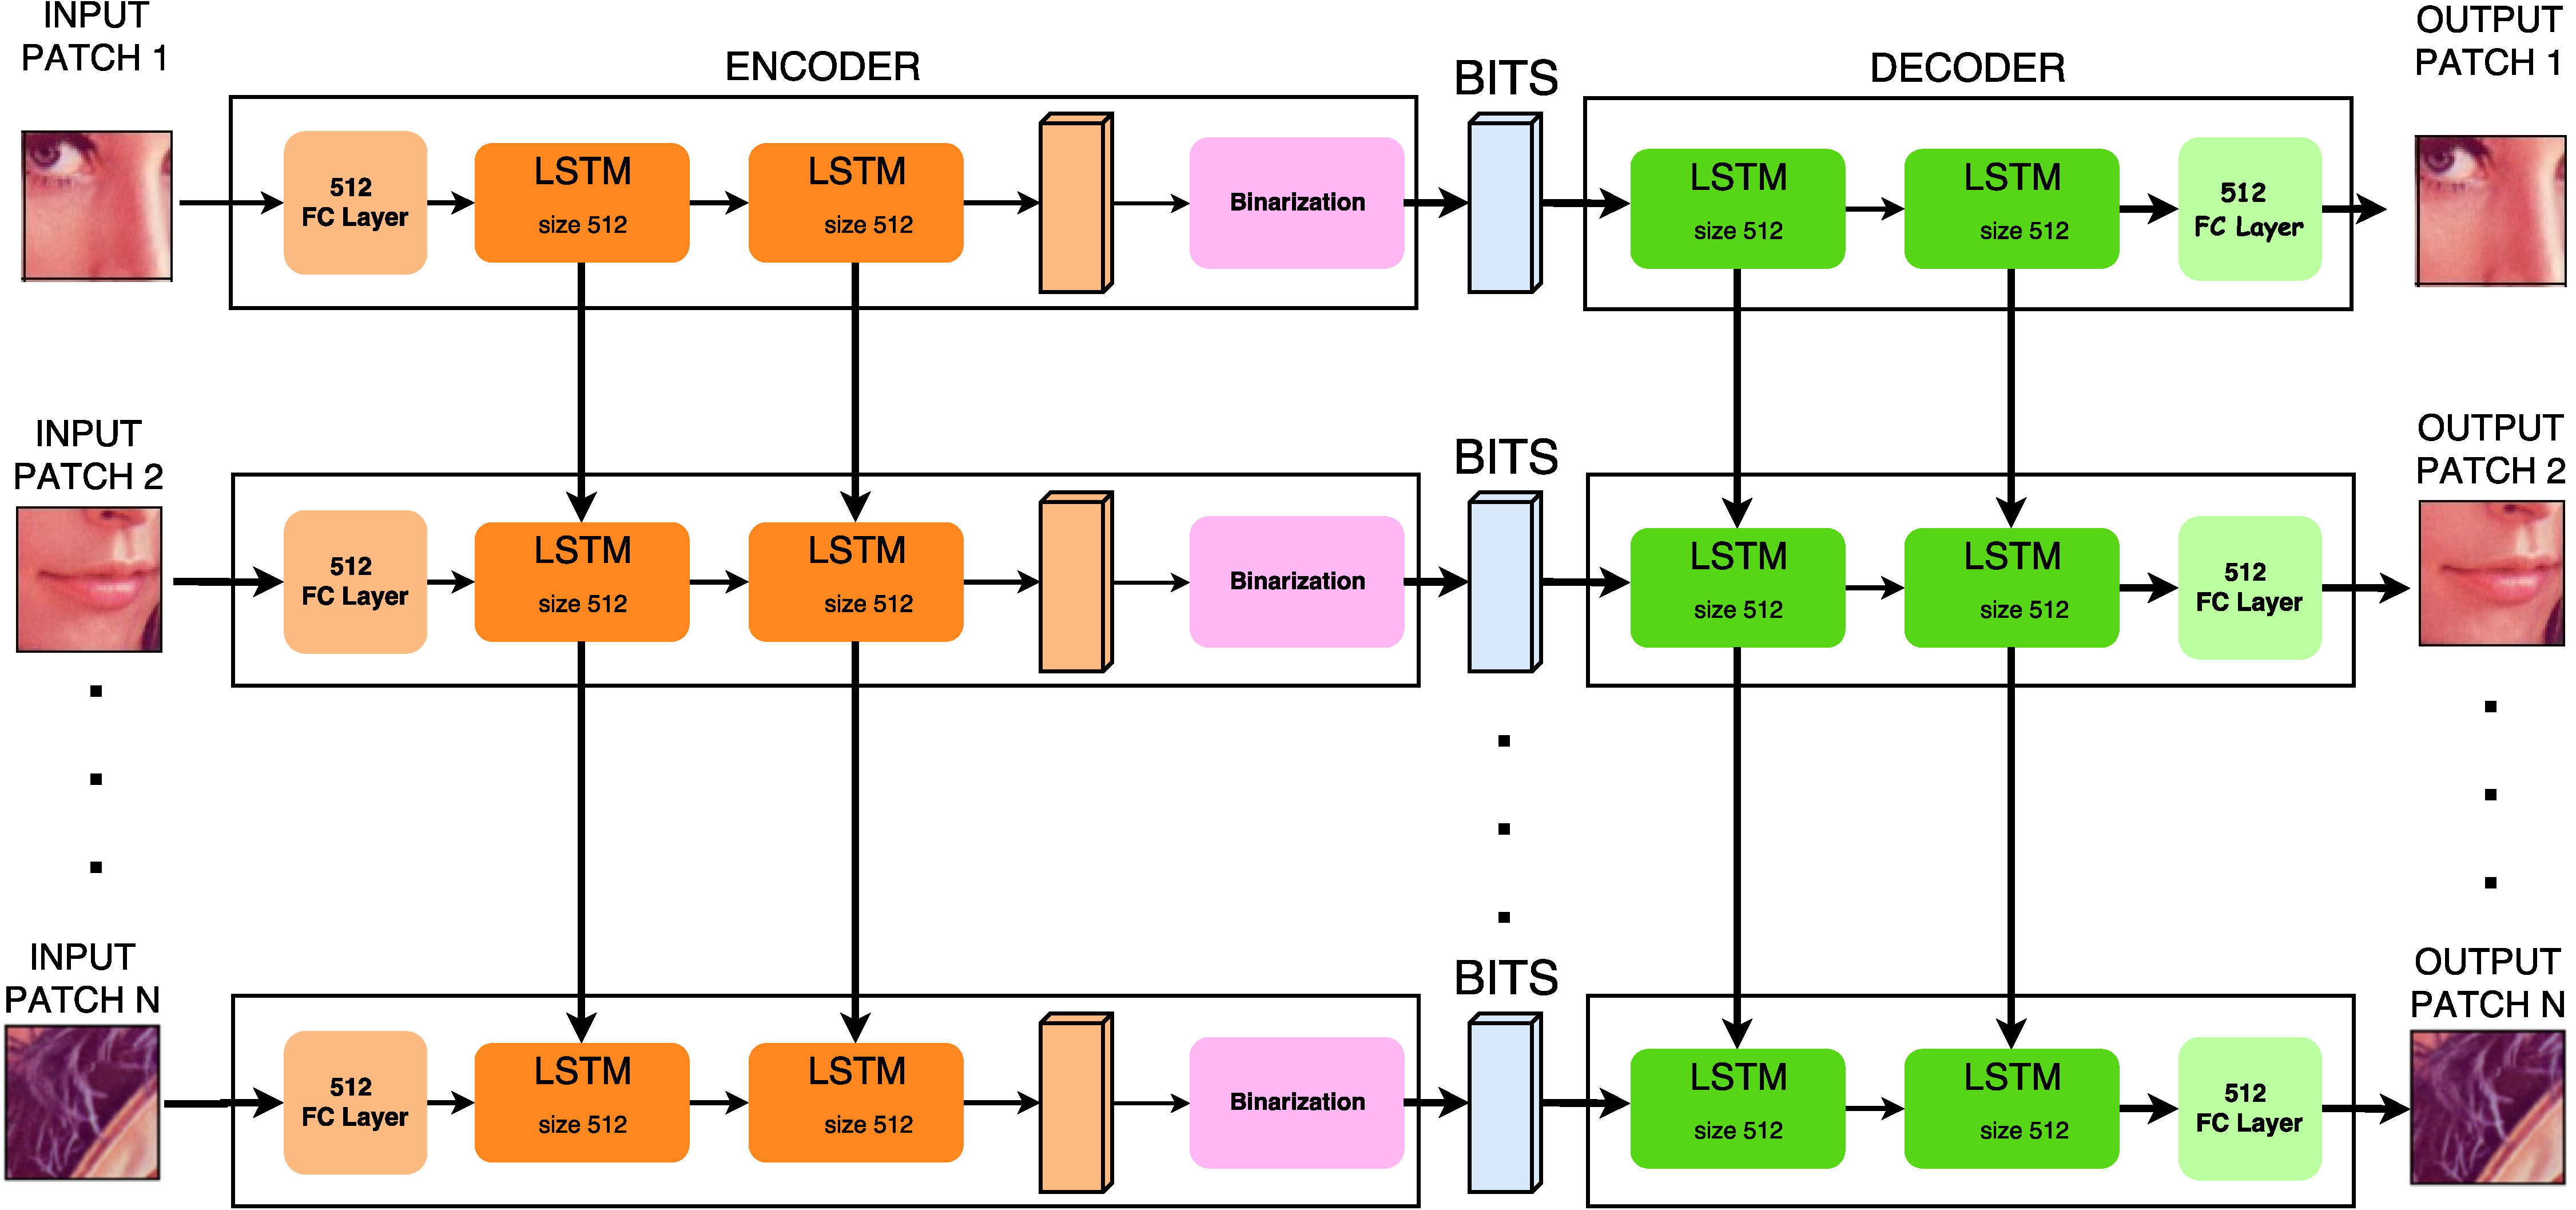
\includegraphics[width=\linewidth]{./img/Our_LSTM.pdf}
  \end{center}
\end{frame}




  % SECTION 5:==================================================================

  \begingroup
  \setbeamercolor{section title}{fg=white}
  \setbeamercolor{background canvas}{bg=mDarkTeal}
  \section{Results}
  \endgroup

  % SLIDE : ____________________________________________________________________
  \begin{frame}{Results: Resources Used}

  \begin{itemize}
    \item Framework: \\
      \begin{center}
        
\includegraphics[width=0.3\linewidth]{./img/python_logo.png}\ 
\includegraphics[width=0.6\linewidth]{./img/pytorch_logo.png}
      \end{center}
    \item Computation: \\
      \begin{center}
        
\includegraphics[width=0.50\linewidth]{./img/AWS_logo.png}
      \end{center}
    \item Dataset: \textit{CIFAR10} and \textit{CIFAR100}\\
    \begin{center}
      
\includegraphics[width=0.6\linewidth]{./img/UoT_logo.png}
    \end{center}
  \end{itemize}

  \end{frame}



  % SLIDE : ____________________________________________________________________
  \begin{frame}{Results: Results Overview}
    \begin{enumerate}
      \item Straight-Forward Fully-Connected
      \item Resiudal Fully-Connected
        \begin{itemize}
          \item 16 bpp (2048 B)
          \item 4 bpp (512 B)
          \item 1 bpp (128 B)
          \item 0.5 bpp (64 B)
        \end{itemize}
      \item Convolutional and Residual Convolutional
      \item Our LSTM
    \end{enumerate}
  \end{frame}


  % SLIDE : ____________________________________________________________________
  \begin{frame}{Results: Parameters to Adjust}
    \begin{itemize}
      \item Encoder-Decoder scheme
      \item Patch size
      \item Encoded size
      \item Number of passes
      \item Training parameters
    \end{itemize}
  \end{frame}


  % SLIDE : ____________________________________________________________________
  \begin{frame}{Results: Little Quizz}
    What is in the picture?
    \begin{center}
      
\includegraphics[width=0.5\linewidth]{./img/lion_512B.png}
    \end{center}
  \end{frame}
  % SLIDE : ____________________________________________________________________
  \begin{frame}{Results: Little Quizz}
    What is in the picture?
    \begin{center}
      
\includegraphics[width=0.5\linewidth]{./img/lion_512B.png}
      
\includegraphics[width=0.5\linewidth]{./img/lion.png}
    \end{center}
    \vspace{5mm}
    \begin{figure}
      \begin{minipage}{\textwidth}
              \footnotetext{[6] 4bpp (512B) FC Residual decoded (left) and original (right) 32x32 images  } \\
      \end{minipage}
  \end{figure}
  \end{frame}


  % SLIDE : ____________________________________________________________________
  \begin{frame}{Results: Poor-Quality Results Comparison}
    Results comparison using 0.5 bpp:
    \begin{center}
      
\includegraphics[width=0.3\linewidth]{./img/decoded_imgs/dog.png}
      
\includegraphics[width=0.3\linewidth]{./img/decoded_imgs/dog_FC_64B.png}
      
\includegraphics[width=0.3\linewidth]{./img/decoded_imgs/dog_ConvRes_p32_b64-p8.png}\\
      
\includegraphics[width=0.3\linewidth]{./img/decoded_imgs/dog_LSTM.png}
      
\includegraphics[width=0.3\linewidth]{./img/decoded_imgs/dog_64B.png}
    \end{center}
    \begin{figure}
      \begin{minipage}{\textwidth}
              \footnotetext{[7] From top-left to bottom-right:\\ Original, FC, Convolutional Residual, Our LSTM, FC Resiudal    } \\
      \end{minipage}
  \end{figure}
  \end{frame}

  % SLIDE : ____________________________________________________________________
  \begin{frame}{Results: Poor-Quality Results Comparison}
    Results comparison using 0.5 bpp:
    \begin{center}
      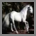
\includegraphics[width=0.3\linewidth]{./img/decoded_imgs/horse.png}
      
\includegraphics[width=0.3\linewidth]{./img/decoded_imgs/horse_FC_64B.png}
      
\includegraphics[width=0.3\linewidth]{./img/decoded_imgs/horse_ConvRes_p32_b64-p8.png}\\
      
\includegraphics[width=0.3\linewidth]{./img/decoded_imgs/horse_LSTM.png}
      
\includegraphics[width=0.3\linewidth]{./img/decoded_imgs/horse_64B.png}
    \end{center}
    \begin{figure}
      \begin{minipage}{\textwidth}
              \footnotetext{[8] From top-left to bottom-right:\\ Original, FC, Convolutional Residual, Our LSTM, FC Resiudal    } \\
      \end{minipage}
  \end{figure}
  \end{frame}

  % SLIDE : _____________________________________________________________________
  \begin{frame}{Results: Poor-Quality Results Comparison}

    \begin{center}
      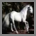
\includegraphics[width=0.2\linewidth]{./img/decoded_imgs/horse.png}
      
\includegraphics[width=0.2\linewidth]{./img/decoded_imgs/horse_FC_64B.png}
      
\includegraphics[width=0.2\linewidth]{./img/decoded_imgs/horse_ConvRes_p32_b64-p8.png}
      
\includegraphics[width=0.2\linewidth]{./img/decoded_imgs/horse_LSTM.png}
      
\includegraphics[width=0.2\linewidth]{./img/decoded_imgs/horse_64B.png}
    \end{center}
    \vspace{10mm}
    \begin{center}
      \resizebox{0.95\columnwidth}{!}{%
\begin{tabular}{|l|c|c|c|c|}
\hline
     & FC & Convolutional Residual & Our LSTM  & FC Residual    \\
\hline
SSIM & 0.7844 & 0.6932 & 0.6520 & 0.8191  \\
\hline
MSE &77.942 & 79.370 & 81.64 & 77.527   \\
\hline
\end{tabular}%
}
\end{center}
\vspace{20mm}
\begin{figure}
  \begin{minipage}{\textwidth}
          \footnotetext{[9] Scores shown are the average value over a pre-defined set of 20 random pictures\\ \\
          Pictures from right to left: Original, FC, Convolutional Residual, Our LSTM and FC Residual} \\
  \end{minipage}
\end{figure}

  \end{frame}



  % SLIDE : _____________________________________________________________________
  \begin{frame}{Results: FC Residual Analysis}
    \begin{center}
      
\includegraphics[width=0.3\linewidth]{./img/decoded_imgs/dog.png}
      
\includegraphics[width=0.3\linewidth]{./img/decoded_imgs/dog_64B.png}
      
\includegraphics[width=0.3\linewidth]{./img/decoded_imgs/dog_128B.png}\\
      
\includegraphics[width=0.3\linewidth]{./img/decoded_imgs/dog_512B.png}
      
\includegraphics[width=0.3\linewidth]{./img/decoded_imgs/dog_2048B.png}
    \end{center}
    \begin{figure}
      \begin{minipage}{\textwidth}
              \footnotetext{[10] From top-left to bottom-right: Original, 0.5 bpp, 1 bpp, 4 bpp & 16 bpp } \\
      \end{minipage}
  \end{figure}
  \end{frame}
  % SLIDE : _____________________________________________________________________
  \begin{frame}{Results: FC Residual Analysis}
    \begin{center}
      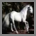
\includegraphics[width=0.3\linewidth]{./img/decoded_imgs/horse.png}
      
\includegraphics[width=0.3\linewidth]{./img/decoded_imgs/horse_64B.png}
      
\includegraphics[width=0.3\linewidth]{./img/decoded_imgs/horse_128B.png}\\
      
\includegraphics[width=0.3\linewidth]{./img/decoded_imgs/horse_512B.png}
      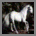
\includegraphics[width=0.3\linewidth]{./img/decoded_imgs/horse_2048B.png}
    \end{center}
    \begin{figure}
      \begin{minipage}{\textwidth}
              \footnotetext{[11] From top-left to bottom-right: Original, 0.5 bpp, 1 bpp, 4 bpp & 16 bpp } \\
      \end{minipage}
  \end{figure}
  \end{frame}

  % SLIDE : _____________________________________________________________________
  \begin{frame}{Results: FC Residual Analysis}

    \begin{center}
      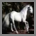
\includegraphics[width=0.2\linewidth]{./img/decoded_imgs/horse.png}
      \includegraphics[width=0.2\linewidth]{./img/decoded_imgs/horse.png}
      \includegraphics[width=0.2\linewidth]{./img/decoded_imgs/horse_128B.png}
      \includegraphics[width=0.2\linewidth]{./img/decoded_imgs/horse_512B.png}
      \includegraphics[width=0.2\linewidth]{./img/decoded_imgs/horse_2048B.png}
    \end{center}

    \begin{center}
\resizebox{0.8\columnwidth}{!}{%
    \begin{tabular}{|c||c||c|c|c|}

  \hline
& JPEG  & \multicolumn{3}{c|}{FC Residual}\\
  \hline
  \hline
BPP & 1.20 & 1 & 4 & 16 \\
  \hline
SSIM & 0.967 & 0.8654 & 0.9478  & 0.9951 \\
\hline
MSE & 30.06 & 74.351 & 64.952  & 20.451 \\
\hline
\end{tabular}%
}
\end{center}
\vspace{10mm}
\begin{figure}
  \begin{minipage}{\textwidth}
          \footnotetext{[12] Scores shown are the average value over a pre-defined set of 20 random pictures\\ \\
          Pictures from right to left: Original, JPEG, FC Resiudual using 1, 4 and 16 bpp } \\
  \end{minipage}
\end{figure}
  \end{frame}




  % SECTION 6:====================================================================

  \begingroup
  \setbeamercolor{section title}{fg=white}
  \setbeamercolor{background canvas}{bg=mDarkTeal}
  \section{Conclusions}
  \endgroup

  % SLIDE : _____________________________________________________________________
  \begin{frame}{Conclusions}
    \begin{itemize}
      \item Low variable bitrate coding acomplish
      \item NN can be applied to image coding
      \item JPEG solid coding scheme and hard to be outperformed
      \item Results obtained are fair for an accademic project
      \item Further improves are needed
    \end{itemize}
  \end{frame}



% ENDING: ======================================================================


\maketitle

\end{document}
